%%%%%%%%%%%%%%%%%%%%%%%%%%%%%%%%%%%%%%%%%%%%%%%%%%%%%%%%%%%%%%%%%%%%%%
% LaTeX Template: Beamer arrows
%
% Source: http://www.texample.net/
% Feel free to distribute this template, but please keep the
% referal to TeXample.net.
% Date: Nov 2006
% 
%%%%%%%%%%%%%%%%%%%%%%%%%%%%%%%%%%%%%%%%%%%%%%%%%%%%%%%%%%%%%%%%%%%%%%
% How to use writeLaTeX: 
%
% You edit the source code here on the left, and the preview on the
% right shows you the result within a few seconds.
%
% Bookmark this page and share the URL with your co-authors. They can
% edit at the same time!
%
% You can upload figures, bibliographies, custom classes and
% styles using the files menu.
%
% If you're new to LaTeX, the wikibook is a great place to start:
% http://en.wikibooks.org/wiki/LaTeX
%
%%%%%%%%%%%%%%%%%%%%%%%%%%%%%%%%%%%%%%%%%%%%%%%%%%%%%%%%%%%%%%%%%%%%%%

\documentclass{beamer} %
\usetheme{Warsaw}
\usepackage[latin1]{inputenc}
\usefonttheme{professionalfonts}
\usepackage{times}
\usepackage{amsmath}
\usepackage{verbatim}

\usepackage{graphicx}

\author{Fernando Pujaico Rivera and Roberto Alves Braga}
\title{BSL Sound}

\usepackage{multimedia}
\begin{document}


%%%%%%%%%%%%%%%%%%%%%%%%%%%%%%%%%%%%%%%%%%%%%%%%%%%%%%%%%%%%%%%%%%%%%%%%%%%%%%%%
\frame{\titlepage}

%%%%%%%%%%%%%%%%%%%%%%%%%%%%%%%%%%%%%%%%%%%%%%%%%%%%%%%%%%%%%%%%%%%%%%%%%%%%%%%%
% \begin{frame}
% \frametitle{Table of Contents}
% \tableofcontents[currentsection]
% \end{frame}

%%%%%%%%%%%%%%%%%%%%%%%%%%%%%%%%%%%%%%%%%%%%%%%%%%%%%%%%%%%%%%%%%%%%%%%%%%%%%%%%
\begin{frame}
\frametitle{Model}
\begin{center}
 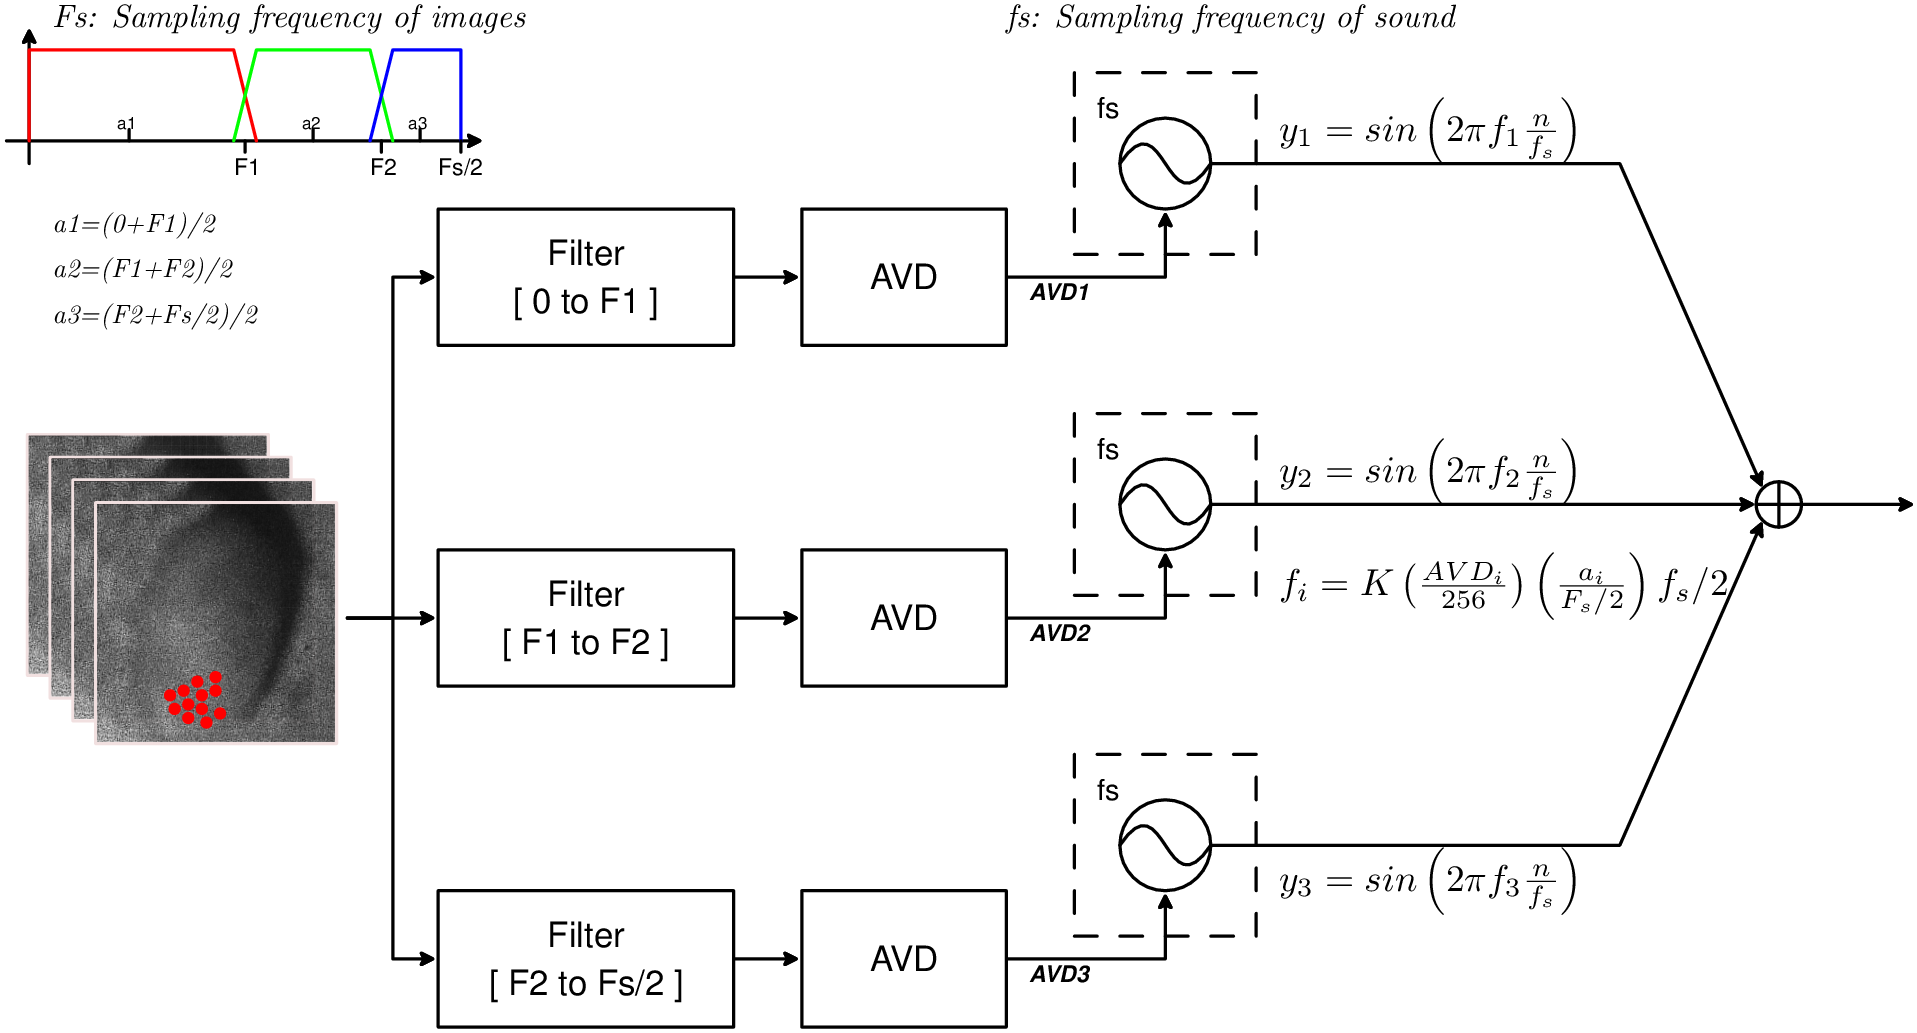
\includegraphics[width=0.95\textwidth]{./images/Diagrama1.png}
\end{center}
\end{frame}

%%%%%%%%%%%%%%%%%%%%%%%%%%%%%%%%%%%%%%%%%%%%%%%%%%%%%%%%%%%%%%%%%%%%%%%%%%%%%%%%
\begin{frame}
\frametitle{explanation}
\begin{equation*}
F_1=\frac{4}{7}\frac{F_s}{2},~~F_2=\frac{6}{7}\frac{F_s}{2},~~\frac{F_s}{2}=4Hz
\end{equation*}
\begin{equation*}
 K=4,~~f_s=8000Hz
\end{equation*}

\begin{columns}
\begin{column}{0.5\textwidth}
\sound[inline,autostart]{Play the sound clicking in:}{low_activity.mp3}
low\_activity.mp3
    \begin{center}
     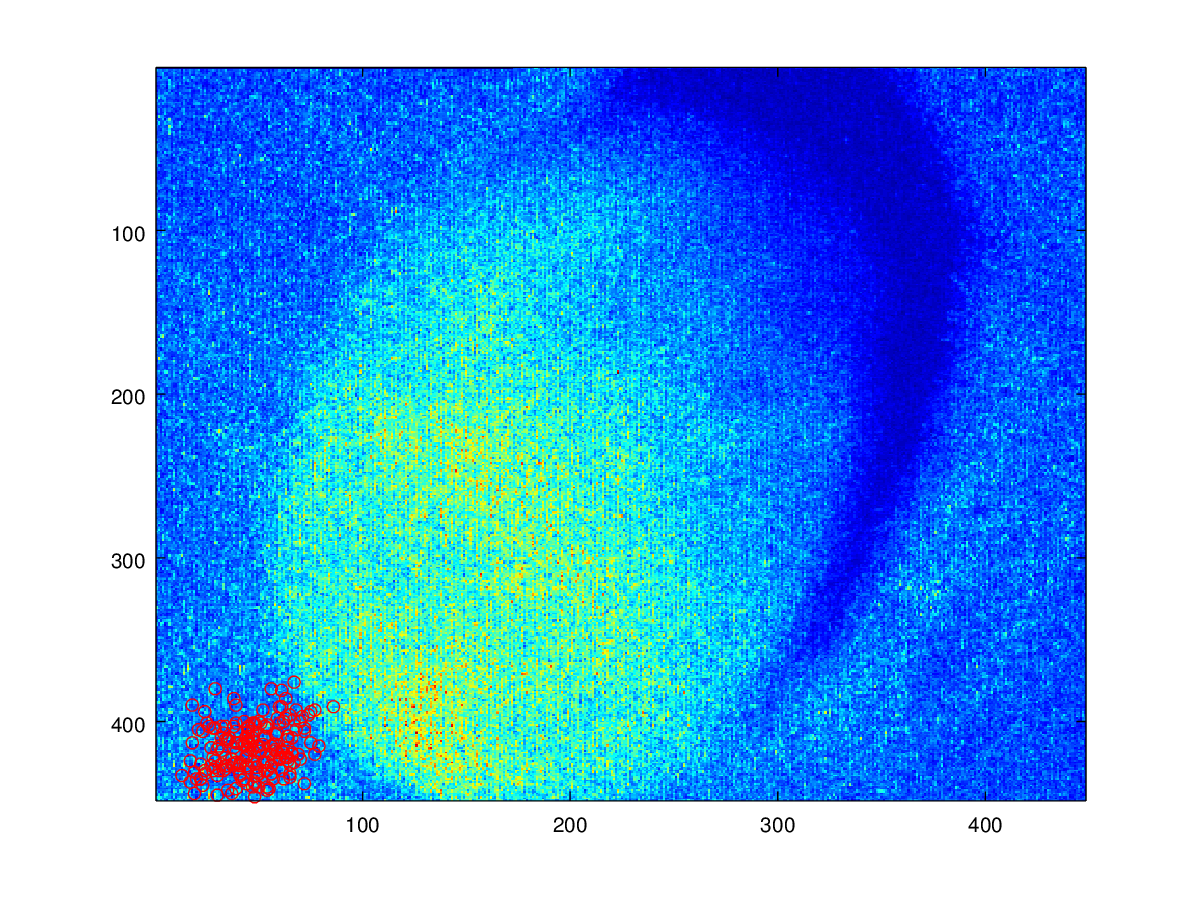
\includegraphics[width=0.95\textwidth]{images/slected_points_low.png}
     \end{center}
\end{column}
\begin{column}{0.5\textwidth}  %%<--- here
\sound[inline,autostart]{Play the sound clicking in:}{high_activity.mp3}
high\_activity.mp3
    \begin{center}
     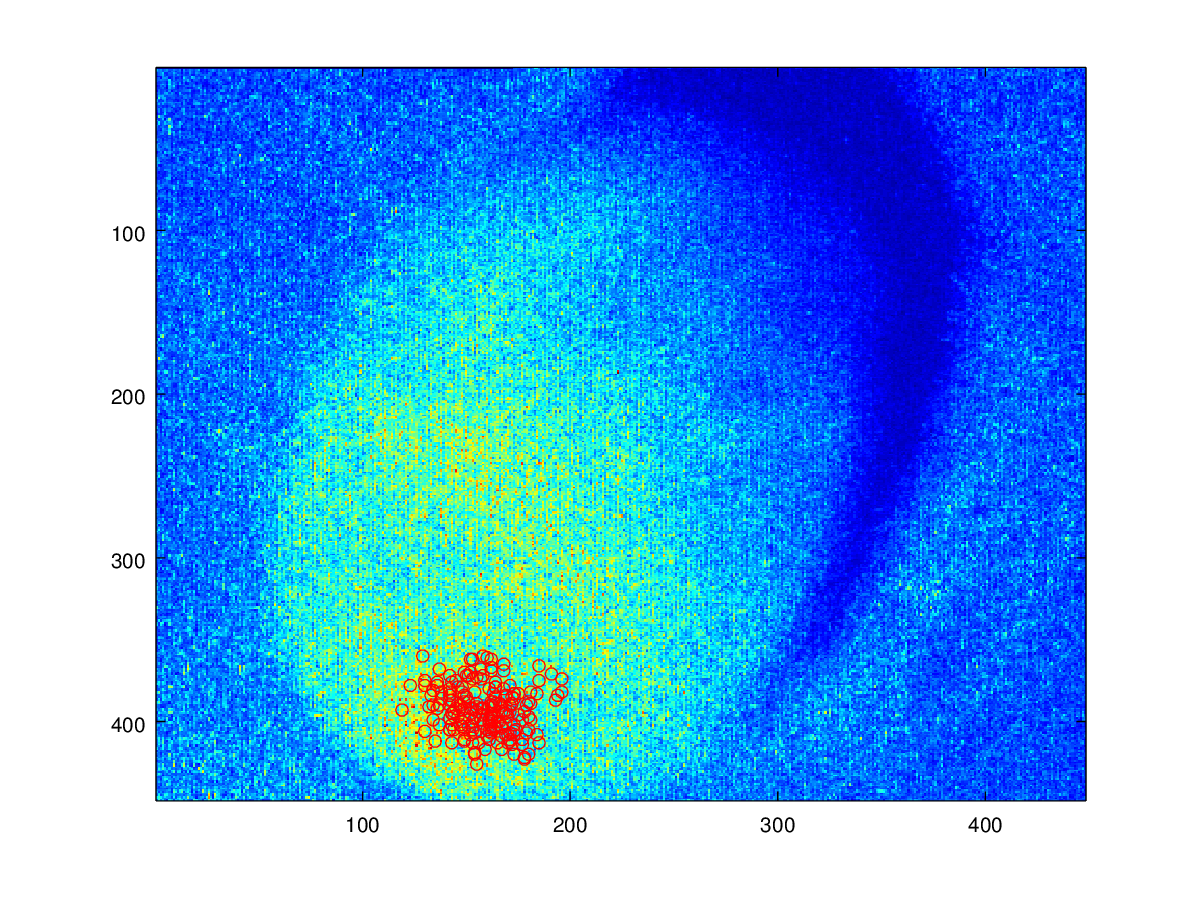
\includegraphics[width=0.95\textwidth]{images/slected_points_high.png}
     \end{center}
\end{column}
\end{columns}
\end{frame}




\end{document}